\section{研究问题}

%%%%%%%%%%%%%%%
% \begin{frame}{分布数据一致性问题}
%   \graphicspath{{tikz-in-beamer/}}
%   \begin{figure}[h!]
%     \centering
%     \begin{adjustbox}{max totalsize = {0.50\textwidth}{1.00\textheight}, center}
% 	  % File: beamer overlay for distributed-data.tex
% Created: Nov. 2, 2016

\begin{tikzpicture}[rc/.style = {circle, minimum size = 4cm, fill = red},
  br/.style = {rectangle, rounded corners, minimum size = 4cm, fill = blue},
  gs/.style = {shape = star, scale = 8, star points = 5, star point ratio = 1.65, fill = green},
  dash pattern = {on 20pt off 10pt},
  partition/.style = {draw, lightgray, line width = 8pt},
  replication/.style = {draw, dash phase = 0pt, line width = 10pt, #1},
  access/.style = {draw, > = stealth, <->, dash phase = 0pt, line width = 6pt, brown}]

  \begin{pgfonlayer}{background}
	\node[opacity = 0.80] (map) {\includegraphics[scale = 0.50]{figs/world-map-logo.jpg}};
  \end{pgfonlayer}

  % shared data
  \begin{scope}[yshift = -18cm]
	\node[rc] (circ) {};
	\node[br, left = 2cm of circ] (rect) {};
	\node[gs, right = 2cm of circ] (st) {};

	\begin{pgfonlayer}{background}
	  \node[rectangle, rounded corners, fill = black!30, fit = (circ) (rect) (st), inner sep = 5pt, 
		label = {[font = \fontsize{65}{70}\sffamily\bfseries] below : Application Data}] (data) {};
	  \end{pgfonlayer}
	\end{scope}

	% partition
	\node[rc] (circ1) at (20, 10) {};
	\node[br] (rect1) at (-25, 10) {};
	\node[gs] (st1) at (28, -12) {};

	\draw[partition] (circ) to (circ1);
	\draw[partition] (rect) to (rect1);
	\draw[partition] (st) to (st1);


	% replication
	\node[rc] (circ2) at (-15, -10) {};
	\node[rc] (circ3) at (-10, 18) {};

	\node[br] (rect2) at (10, 12) {};

	\node[gs] (st2) at (0,0) {};
	\node[gs] (st3) at (20, 5) {};

	\path[replication = {red}] (circ1) to (circ2) 
	(circ2) to (circ3)
	(circ3) to (circ1);

	\path[replication = {blue}] (rect1) to (rect2);

	\path[replication = {green}] (st1) to (st2) 
	(st2) to (st3)
	(st3) to (st1);


  \uncover<2->{
  % sina-weibo clients
  \def\SCALE{0.15}
  \node[] (sina1) at (-25, 0) {
\includegraphics[scale = \SCALE]{figs/sina-weibo.png}};
  \node[] (sina2) at (10, 5) {
\includegraphics[scale = \SCALE]{figs/sina-weibo.png}};
  \node[] (sina3) at (5, -10) {
\includegraphics[scale = \SCALE]{figs/sina-weibo.png}};

  % access
  \path[every edge/.append style = {access}] (sina1) edge (rect1)
  				(sina1) edge (circ2)
				(sina2) edge (rect2)
				(sina2) edge (st2)
				(sina3) edge (circ1)
				(sina3) edge (st2);
  }
\end{tikzpicture}

%     \end{adjustbox}
%   \end{figure}
% 
%   \uncover<2->{
% 	\textcolor{red}{分布数据 \term{distributed data}} $\Leftarrow$ 共享 (集中式) 数据 \term{shared data}:}
%   \vspace{0.30cm}
%   \begin{description}
% 	\item<3->[上层应用:] 分布数据的语义是什么? 如何``方便''地使用分布数据?
% 	\item<4->[数据副本:] 以何种顺序应用更新? 对应用提供什么保证?
%   \end{description}
% \end{frame}
% %%%%%%%%%%%%%%%
% \begin{frame}{分布数据一致性问题}
%   \begin{figure}[h!]
%     \centering
%     \begin{adjustbox}{max totalsize = {0.70\textwidth}{1.00\textheight}, center}
% 	  % This example is from WYATT LLOYD@CACM14 (Don't Settle For Eventual Consistency)
\begin{tikzpicture}
  % replica A at west coast
  \begin{scope}[font = \Large, wnode/.style = {fill = blue!60, circle}]
    \node (west-start) [] at (0,0) {};
    \node (west-end) [below = 8cm of west-start] {};

	\uncover<2->{
    \draw [>=Stealth, ->, ultra thick] (west-start) to (west-end);

    \node (west-a-lost) [wnode, label = 180: $A_{\textrm{lost}}$] at ($(west-start) !0.10! (west-end)$) {};
    \node (west-a-found) [wnode, label = 180: $A_{\textrm{found}}$] at ($(west-start) !0.30! 
    (west-end)$) {};
    \node (west-b-glad) [wnode, label = 180: $B_{\textrm{glad}}$] at ($(west-start) !0.60! (west-end)$) {};

    % text
    \node (west-text) [above left = 1.5cm and -3.00cm of west-start, align = center, font = \LARGE] {{\bf A}lice: I've {\bf lost} my ring.
    \\ $\qquad$ {\bf A}lice: I {\bf found} it upstairs. 
    \\ $\qquad$ {\bf B}ob: {\bf Glad} to hear that.};
  }

    % replica A at west coast
	\uncover<1->{
	  \node (replicaA) [above = -0.20cm of west-start, font = \LARGE, draw = blue, rectangle, rounded corners] {\textcolor{blue}{Replica A}};}
  \end{scope}

  % replica B at east coast
  \begin{scope}[xshift = 8.0cm, font = \Large, enode/.style = {fill = brown!60, circle}]
    \node (east-start) [] at (0,0) {};
    \node (east-end) [below = 8cm of east-start] {};
	\uncover<3->{
	\draw [>=Stealth, ->, ultra thick] (east-start) to (east-end);

    \node (east-a-lost) [enode, label = 0: $A_{\textrm{lost}}$] at ($(east-start) !0.20! (east-end)$) {};
    \node (east-b-glad) [enode, label = 0: $B_{\textrm{glad}}$] at ($(east-start) !0.40! 
    (east-end)$) {};
    \node (east-a-found) [enode, label = 0: $A_{\textrm{found}}$] at ($(east-start) !0.85! (east-end)$) {};

  % message-passing and message-reordering
  \begin{scope}[>=Stealth, ->, thick, dashed, red]
    \draw (west-a-lost) to (east-a-lost);
    \draw (west-a-found) to (east-a-found);
    \draw (west-b-glad) to (east-b-glad);
  \end{scope}
  }
    
    % replica B at east coast
	\uncover<1->{
	  \node (replicaB) [above = -0.20cm of east-start, font = \LARGE, draw = brown, rectangle, rounded corners] {\textcolor{brown}{Replica B}};}
  \end{scope}

  \uncover<4->{
  \begin{scope}[font = \Large]
    % data inconsistency in replicaB
    \draw [line width = 5pt, red] (east-b-glad) -- (east-a-found) 
	node (inconsistency) [above, midway, sloped, outer sep = 5pt] {inconsistency};
    % text
    \node (east-text) [draw = red, very thick, rectangle, 
	above right = 1.5cm and -3.00cm of east-start, align = center, font = \LARGE, 
	  outer sep = 5pt] 
	  {{\bf A}lice: I've {\bf lost} my ring.  
	  \\ $\qquad$ {\bf B}ob: {\bf Glad} to hear that.};
	% link
    \draw [>=Stealth, very thick, red, <->] 
	  (inconsistency) -| ($(east-text.south) + (30pt,0)$);
  \end{scope}
  }
\end{tikzpicture}

%     \end{adjustbox}
% 	\caption{社交网络中, 消息-评论乱序 \citeinbeamer{Lloyd}{CACM}{14}.}
%   \end{figure}
% \end{frame}
%%%%%%%%%%%%%%%
\begin{frame}{分布数据一致性问题}
  \graphicspath{{tikz-in-beamer/}}
  \begin{figure}[h!]
    \centering
    \begin{adjustbox}{max totalsize = {0.90\textwidth}{1.00\textheight}, center}
	  \begin{tikzpicture}[font = \Large]
  \node (share) [label = {below:共享数据}] {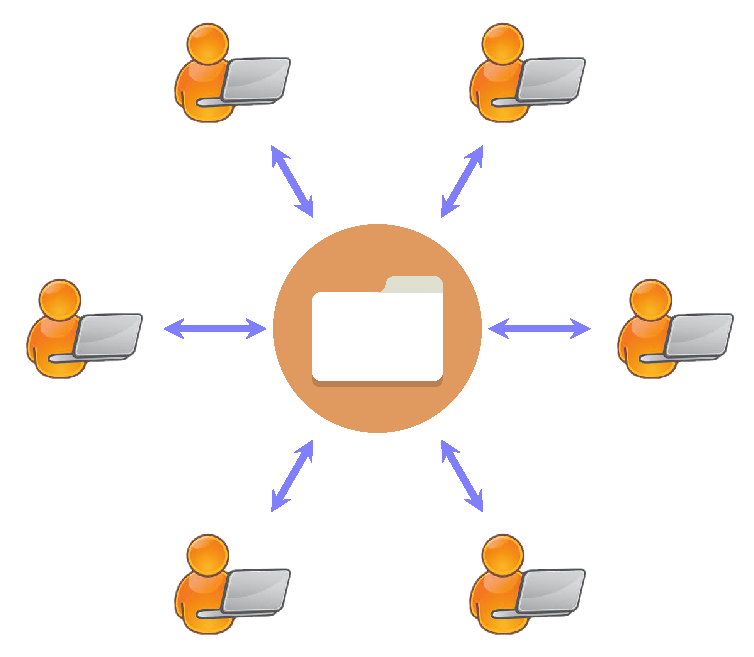
\includegraphics[height = 4cm]{shared-data-clients.pdf}};
  \node (dist) [label = {below:分布数据}, right = 9.0cm of share] {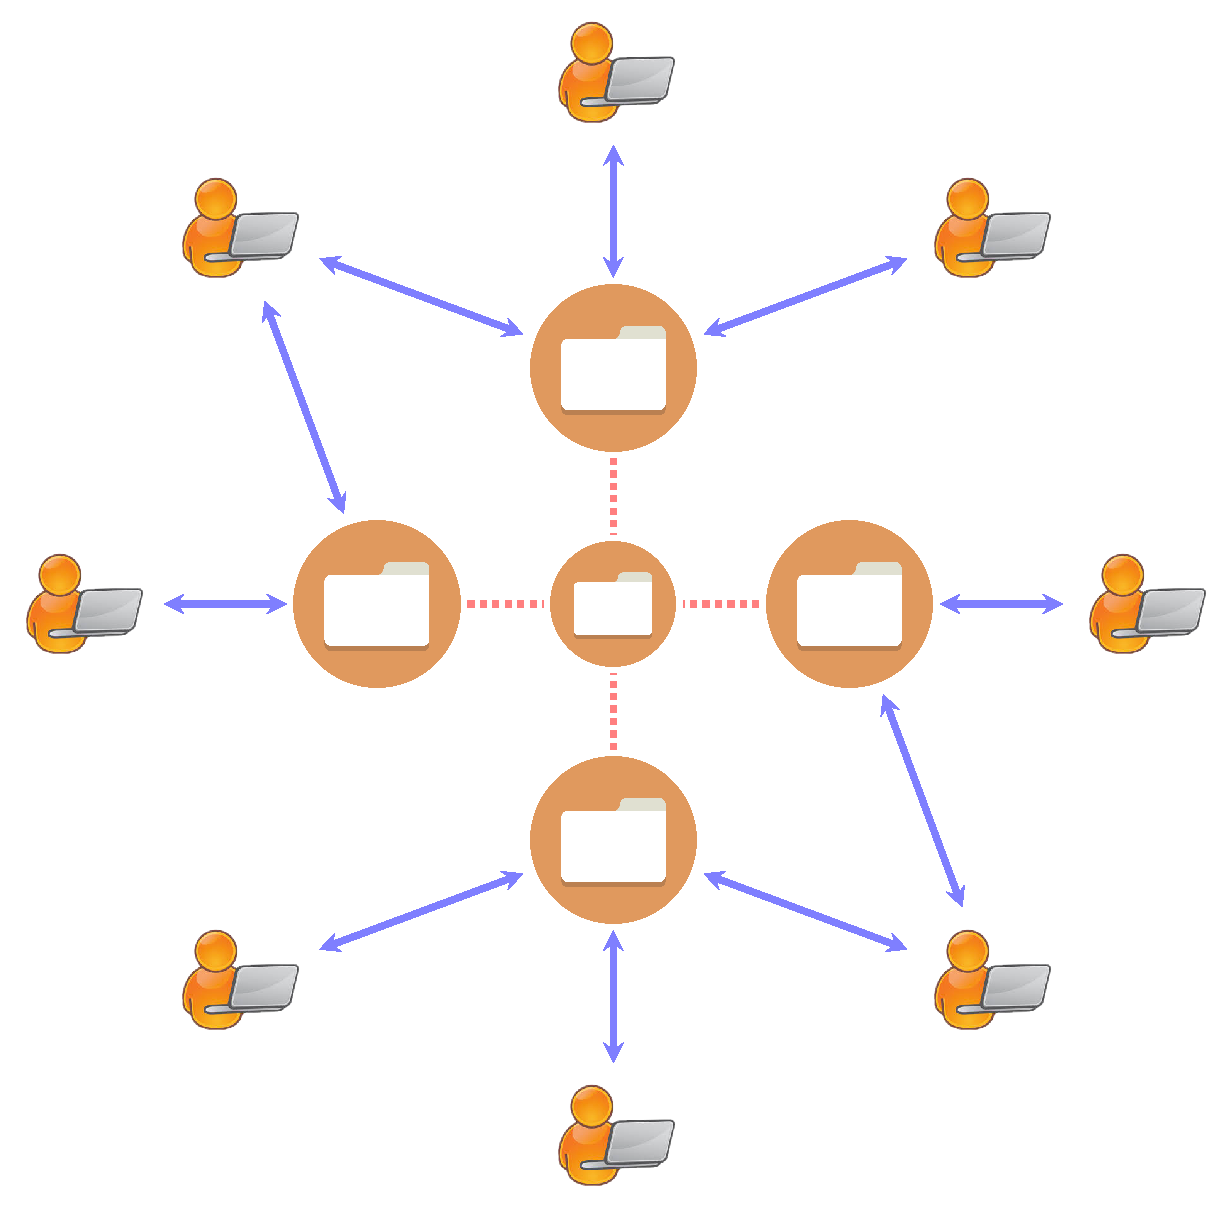
\includegraphics[height = 4.5cm]{distributed-data-clients.pdf}};

  % from (share) to (dist)
  \uncover<2->{
  \draw [-Implies, brown, line width = 1pt, double distance = 2pt, bend right = 35] (share) to node [black, sloped, below = 8pt] {分布数据一致性问题} (dist);
  }

  % from (dist) to (share)
  \uncover<4->{
  \draw [-Implies, brown, line width = 1pt, double distance = 2pt, bend right = 35] (dist) to node () [black, sloped, above = 8pt] 
  {像访问共享数据一样访问分布数据} (share);
  }

  % middleware
  \uncover<3->{
  \node (dsds) [] at ($(share.center)!0.5!(dist.center)$) {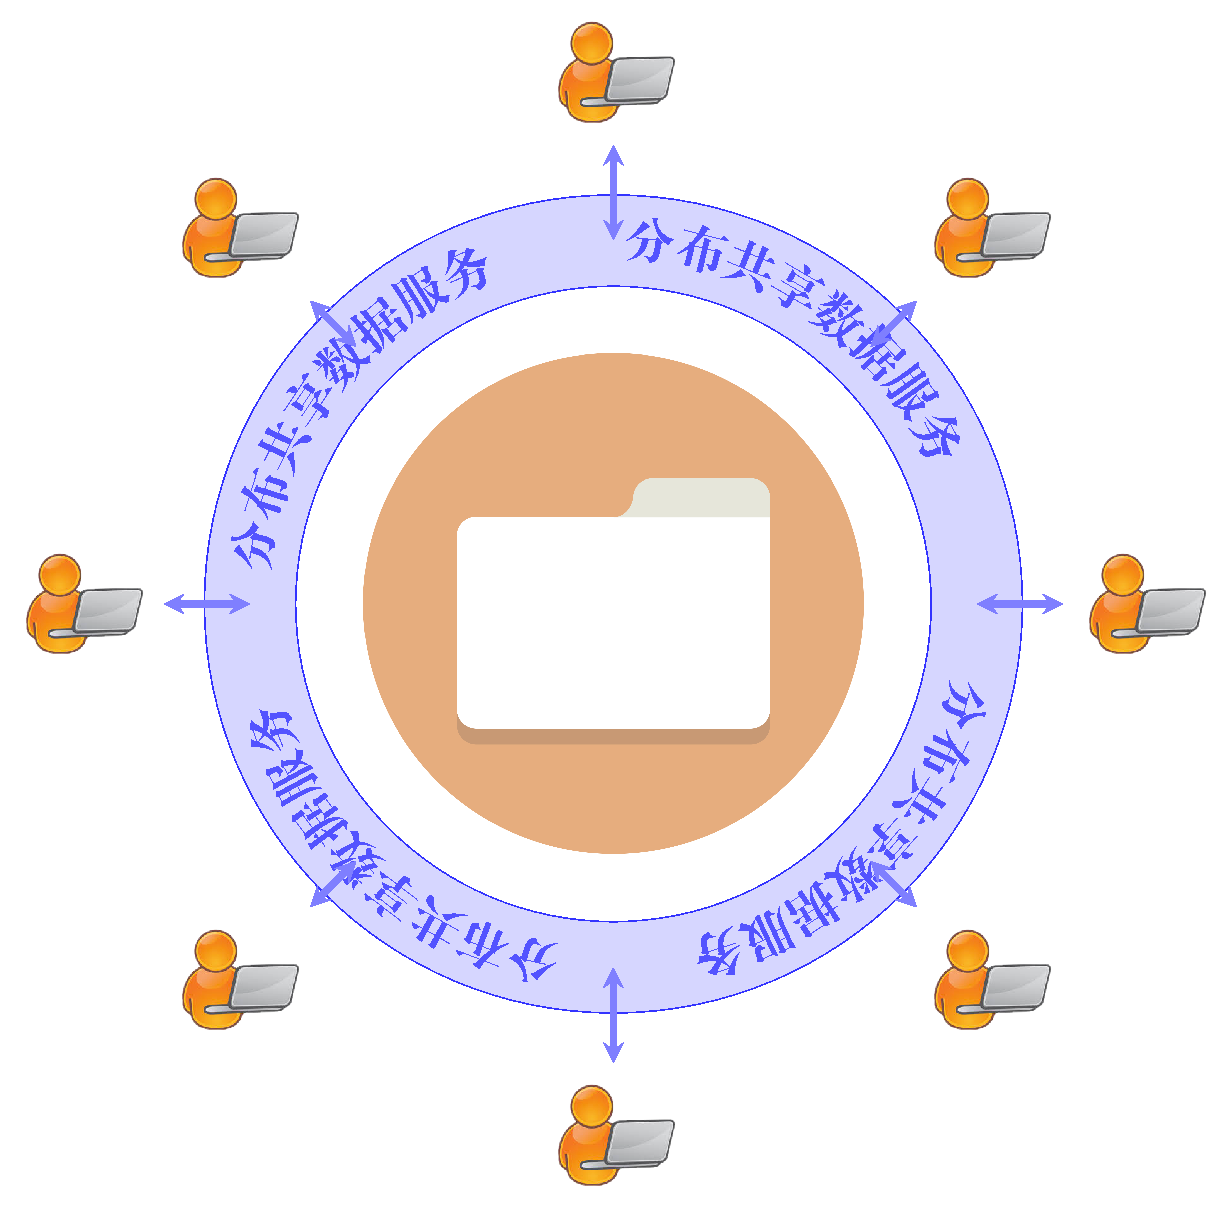
\includegraphics[height = 6cm]{distributed-shared-data-clients-chinese.pdf}};
  \draw [-Implies, blue!60, line width = 1pt, double distance = 1pt] (dist) to (dsds);
  \draw [-Implies, blue!60, line width = 1pt, double distance = 1pt] (dsds) to (share);
  }
\end{tikzpicture}
    \end{adjustbox}
  \end{figure}

  \begin{columns}
	\column{0.50\textwidth}
	  \uncover<2->{
		分布数据一致性问题 \textcolor{blue}{\small (应用视角)}:
	  \begin{itemize}
		\item 分布数据的语义是什么?
		\item 如何``方便''地使用分布数据?
	  \end{itemize}
	  }
	\column{0.50\textwidth}
	  \uncover<3->{
		分布共享数据服务 \textcolor{blue}{\small (中间件)}:
		\begin{itemize}
		  \item 屏蔽分布数据细节
		  \item 提供共享数据抽象
		\end{itemize}
	  }
  \end{columns}
\end{frame}
%%%%%%%%%%%%%%%
\begin{frame}{分布数据一致性问题}
  \begin{columns}[t]
	\column{0.40\textwidth}
	  理想情况:
	  \begin{itemize}
		\item one-size-fits-all\\一致性方案
		\item 始终观察到最新副本
	  \end{itemize}
	  \only<1-2>{
	  \begin{center}
		\textcolor{blue}{没有分布数据一致性问题}
	  \end{center}
	  }
	  \only<3->{
	  \begin{center}
		\textcolor{blue}{\soutthick{没有分布数据一致性问题}}
	  \end{center}
	  }
    \pause
	\column{0.48\textwidth}
	实际情况 (tradeoffs):
	  \fignocaption{width = 0.60\textwidth}{figures/consistency-centric-tradeoff.pdf}
  \end{columns}
  \pause
  \vspace{0.50cm}
  \begin{center}
	% \textcolor{red}{分布数据一致性问题是分布共享数据服务中的核心问题}
	\textcolor{blue}{在大规模分布式系统中, \\以数据一致性为核心的权衡 \citeinbeamer{Guerraoui}{TCDE}{16} 使得 \\
  		分布数据一致性问题成为分布共享数据服务中的核心难题.}
  \end{center}
\end{frame}
%%%%%%%%%%%%%%%
% \begin{frame}{分布数据一致性问题举例 (I)}
%   \fig{width = 0.60\textwidth}{figures/data-inconsistency-comment-reordering.pdf}
%   {社交网络中, 消息-评论乱序 \citeinbeamer{Lloyd}{CACM}{14}.}
% \end{frame}
% %%%%%%%%%%%%%%%
% \begin{frame}{分布数据一致性问题举例 (II)}
%   \begin{figure}[h!]
%     \centering
%     \begin{adjustbox}{max totalsize = {0.65\textwidth}{0.65\textheight}, center}
%       %        File: data-inconsistency-rmw.tex
%     Created: Thu Oct 08 10:00 AM 2015 C
% Last Change: Thu Oct 08 10:00 AM 2015 C
%
\begin{tikzpicture}
  \uncover<1->{
  \begin{scope}
    % phone
    \node (phone) [] at (0,0) {
\includegraphics[scale = 0.4]{figures/phone-icon.png}};
    % tablet
    \node (tablet) [below left = 4.0cm and 3.0cm of phone] {
\includegraphics[scale = 
    0.55]{figures/tablet-icon.jpg}};
    % pc
    \node (pc) [below right = 4.0cm and 3.0cm of phone] {
\includegraphics[scale = 
    0.60]{figures/pc-icon}};
  \end{scope}
  }

    % write from pc 
  \uncover<2->{
    \begin{scope}[<->, blue, line width = 6pt, font = \huge]
      % person at pc
      \only<2>{
      \node (person-pc) [above left = -1.0cm and -2.0cm of pc] {
\includegraphics[scale = 
      0.30]{figures/person-icon}};
      }
      \draw [] (pc.west) to node [midway, sloped, above] {\textbf{1.} update file $f$} 
      (tablet.east);
      \draw [red, loosely dashed] (pc.north) to [out = 90, in = -20] node [midway, sloped, font = 
      \Huge, scale = 2]{$\times$} (phone.east);
      \draw (pc) to [loop, out = 60, in = -10, looseness = 3] node [midway, above, sloped] 
      {\textbf{1.} update file $f$} (pc);
    \end{scope}
   }


    % read from phone
   \uncover<3->{
    \begin{scope}[<->, brown, line width = 6pt, font = \huge]

      % person at phone
      \node (person-phone) [above left = -1.0cm and -2.0cm of phone] {
\includegraphics[scale = 
      0.30]{figures/person-icon}};

      \draw (phone) to [loop, out = 180, in = -100, looseness = 3] node [midway, below, sloped] 
      {\textbf{2.} read file $f$} (phone);   
    \end{scope}

    % update lost
    \node (inconsistency) [font = \huge, right = of person-phone, red] {\bf Update Lost!};
  }
\end{tikzpicture}

%     \end{adjustbox}
%     \caption{多设备文件共享时, 更新丢失 ($\#N = 3, \#W = 2, \#R = 1$).}
%   \end{figure}
% \end{frame}
%%%%%%%%%%%%%%%
\begin{frame}{分布数据一致性问题}
  \mdf{red}{red}{论文研究动机}{
	\begin{center}
	  \textcolor{teal}{面向大规模分布式系统的\\分布数据一致性理论应体现什么特性?}
	\end{center}
  }

  \pause
  \vspace{0.80cm}

  \begin{center}
	分布式系统设计与其应用有哪些特点,\\对分布数据一致性理论有何影响?
  \end{center}

  % 考察分布数据一致性问题研究的历史:
  % \vspace{8pt}
  % \begin{itemize}
  %   \setlength{\itemsep}{6pt}
  %   \item 核心权衡与解决方案 
  %     \pause
  %   \item 理论与系统
  % \end{itemize}
\end{frame}
%%%%%%%%%%%%%%%
\begin{frame}{多处理器系统领域中的数据一致性理论}
  \textcolor{gray}{\small (分布)} 数据一致性问题是多处理器系统领域中的传统问题:
  \vspace{0.50cm}

  \begin{figure}
	\begin{subfigure}{0.50\textwidth}
	  \centering
	  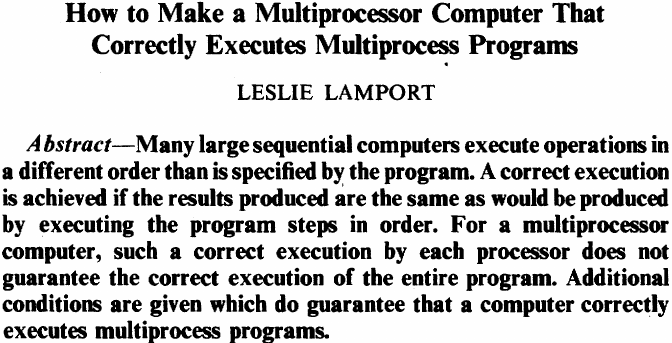
\includegraphics[width = 0.85\textwidth]{figures/lamport-paper79.png}
	  \caption{Sequential Consistency \citeinbeamer{Lamport}{TC}{79}.}
	\end{subfigure}%
	\begin{subfigure}{0.45\textwidth}
	  \centering
	  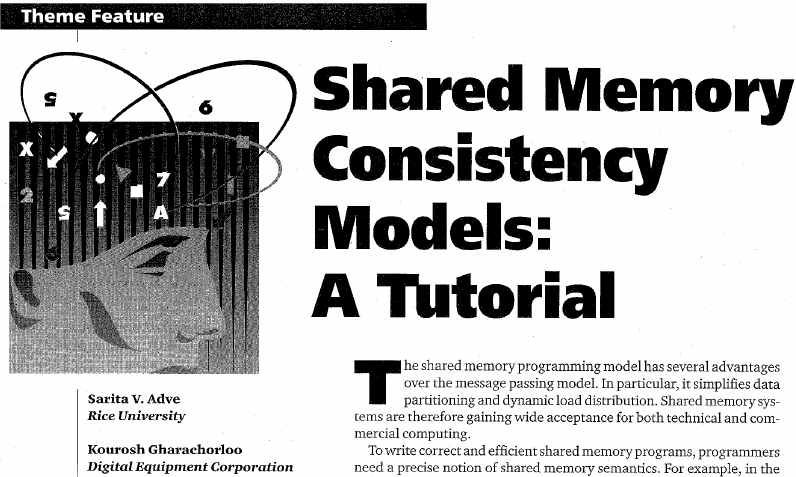
\includegraphics[width = 0.80\textwidth]{figures/ieee-computer-tutorial.png}
	  \caption{Tutorial \citeinbeamer{Adve}{IEEE Computer}{96}.}
	\end{subfigure}
  \end{figure}
\end{frame}
%%%%%%%%%%%%%%%
\begin{frame}{多处理器系统领域中的数据一致性理论}
  \answer{特性: ``以程序为导向、强调正确性''}
  \vspace{0.20cm}

  \begin{description}
	\item[一致性:] 追求``相对于 SC {\small (Sequential Consistency)}''的正确性~\footnotemark[1]~\footnotetext[1]{术语称为 SCNF: Sequential Consistency Normal Form~\citeinbeamer{Adve}{ISCA}{90}.} \citeinbeamer{Adve}{ISCA}{90}
	\item[权衡:] 易编程性 vs. 性能
  \end{description}

	  % \begin{description}
	  %   \item[一致性:] 一致性模型 + 编程模型
	  %   \item[程序:] 遵循预定规则
	  %   \item[系统:] 提供 SC 保证
	  %   \item<3>[权衡:] 易编程性 vs. 性能
	  % \end{description}

  % \fig{width = 0.35\textwidth}{figures/consistency-lattice.png}{一致性模型 {\scriptsize (依据 \citeinbeamer{Steinke}{JACM}{04} 中 Figure~13 重绘)}.}
\end{frame}
%%%%%%%%%%%%%%%
\begin{frame}{分布式系统领域中的数据一致性理论}
  分布数据一致性问题是分布式系统设计的核心问题之一:
  \vspace{0.50cm}

  \begin{figure}
	\begin{subfigure}{0.48\textwidth}
	  \centering
	  \includegraphics[width = 0.90\textwidth]{figures/bayou-paper.png}
	  \caption{Eventual Consistency \citeinbeamer{Terry}{SOSP}{95}.}
	\end{subfigure}%
	\begin{subfigure}{0.48\textwidth}
	  \centering
	  \includegraphics[width = 0.85\textwidth]{figures/dsss.pdf}
	  \caption{分布式存储系统 {\tiny (\textcolor{blue}{左: 开源}; \textcolor{red}{右: 商用})}.} % (\textcolor{blue}{\scriptsize 开源 [左]} \& \textcolor{red}{\scriptsize 商用 [右]})
	\end{subfigure}
  \end{figure}
\end{frame}
%%%%%%%%%%%%%%%
% \begin{frame}{数据一致性问题研究的历史阶段}
%   \fignocaption{width = 0.90\textwidth}{figures/consistency-model-history.pdf}
% 
% \end{frame}
%%%%%%%%%%%%%%%
\begin{frame}{分布式系统领域中的数据一致性理论}
  \answer{更复杂的权衡\only<1-2>{:} \uncover<3->{$\Longrightarrow$ 一致性理论不追求``相对于 SC''的正确性}}

  \fignocaption{width = 0.30\textwidth}{figures/consistency-centric-tradeoff.pdf}
  \vspace{-0.30cm}

  \pause
  \begin{columns}
	\column{0.45\textwidth}
	  \centerline{\textcolor{red}{可用性} vs. 一致性}
	  \vspace{-0.50cm}
	  \fig{width = 0.45\textwidth}{figures/cap-theorem.png}{CAP 定理 \citeinbeamer{Brewer}{PODC}{00}}
	\column{0.50\textwidth}
	  \centerline{\textcolor{red}{访问延迟} vs. 一致性}
	  \vspace{-0.50cm}
	  \fig{width = 0.60\textwidth}{figures/pacelc-tradeoff-new.pdf}{PACELC 权衡 \citeinbeamer{Abadi}{IEEE Computer}{12}}
  \end{columns}
\end{frame}
%%%%%%%%%%%%%%%
\begin{frame}{分布式系统领域中的数据一致性理论}
  \answer{更丰富的应用\only<1>{:} \uncover<2>{$\Longrightarrow$ 一致性理论应体现应用的多样性}}
  \vspace{0.50cm}

  \begin{columns}
	\column{0.45\textwidth}
	\fig{width = 0.75\textwidth}{figures/cassandra-and-datastax.jpg}{Cassandra 分布式存储系统.}
	\column{0.45\textwidth}
	  \fig{width = 0.90\textwidth}{figures/cassandra-datastax-customers.png}{Cassandra \& DataStax 客户.}
  \end{columns}
\end{frame}
%%%%%%%%%%%%%%%
% \begin{frame}{分布式系统领域数据一致性理论}
%   \graphicspath{{tikz-in-beamer/}}
%   \begin{figure}[h!]
%     \centering
%     \begin{adjustbox}{max totalsize = {1.00\textwidth}{1.00\textheight}, center}
% 	  %%%%% Description: beamer overlay for history of (weak) consistency models in the context of distributed systems. %%%%%
%%%%% Date: July 25, 2016 %%%%%
%%%%% Author: Hengfeng Wei (hengxin) %%%%

\begin{tikzpicture}[comment/.style = {align = center},
	axis/.style = {dashed, dash pattern = on 8pt off 4pt, line width = 2pt, draw = red},
	sepline/.style = {dashed, line width = 2pt, opacity = 0.80, blue},
    node distance = 2.0cm]

  %%%%%%%%%% Begin: years and papers %%%%%%%%%% 
  % \x: x coordinate; \y: year; \n: name; \lbl: label
  \foreach \x/\y/\n/\lbl in {
	1/1995/eventual/\textcolor{blue}{Eventual consistency},
	6/2000/cap/\textcolor{red}{\bf CAP theorem},
	12/2006/bigtable/\textcolor{blue}{Bigtable@Google},
	18/2007/dynamo/\textcolor{blue}{Dynamo@Amazon},
	25/2012/pacelc/\textcolor{red}{\bf PACELC tradeoff}} {
	\node[star, star points = 5, minimum size = 3pt, draw = red, fill = yellow, line width = 2pt] (\x) at (\x, 5) {};
	\node[below = 0.50cm of \x, font = \large] (\y) {\bf \y};
	\node[above = 0.50cm of \x, align = center, font = \Large] (\n) {\lbl};
  }

  \path[axis] (1) to (6) to (12) to (18) to (25);
  \draw[> = stealth, ->, axis] (25) to (27, 5);
  %%%%%%%%%% End: decades and systems %%%%%%%%%% 
  \draw[sepline] (8, 1) to (8, 10);
  \draw[sepline] (22, 1) to (22, 10);

  \pause
  %%%%% bayou system %%%%%
  \node[below = of 1995] (bayou-fig) {\includegraphics[scale = 0.35]{figs/bayou-paper.png}};
  \node[above = of eventual] (bayou-eventual) {
\includegraphics[scale = 0.13]{figs/24-7-service.png}};

  %%%%% cap theorem %%%%%
  \node[below = of 2000] (cap-ppt) {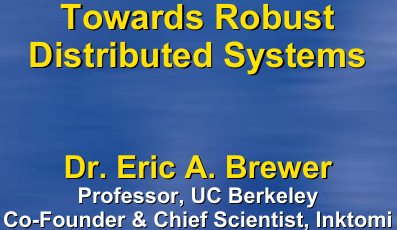
\includegraphics[scale = 0.35]{figs/cap-keynote-ppt.png}};
  % \node[above = of cap] (cap-fig) {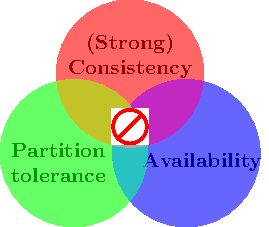
\includegraphics[scale = 0.90]{cap-theorem.pdf}}; 
  \node[above = of cap] (cap-fig) {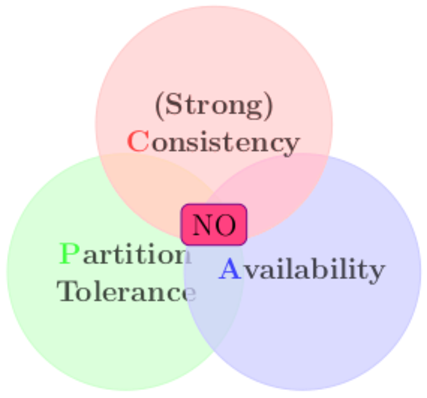
\includegraphics[scale = 0.55]{figs/cap-theorem-no-text.pdf}}; 

  \pause
  %%%%% bigtable %%%%%
  \node[below = of 2006, opacity = 0.80] (bigtable-fig) {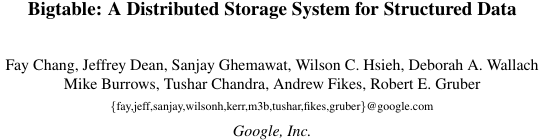
\includegraphics[scale = 0.50]{figs/bigtable-paper.png}};
  \node[above = of bigtable] (bigtable-tradeoff) {
\includegraphics[scale = 0.10]{figs/unavailable.png}};
  
  \pause
  %%%%% dynamo %%%%%
  \node[below = of 2007, opacity = 0.70] (dynamo-fig) {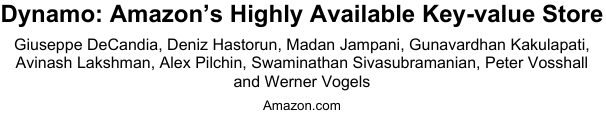
\includegraphics[scale = 0.50]{figs/dynamo-paper.png}};
  \node[above = of dynamo] (dynamo-tradeoff) {
\includegraphics[scale = 0.06]{figs/eventually.jpg}};

  \pause
  %%%%% more systems %%%%%
  \node[] (systems) at ($0.50*(bigtable) + 0.50*(dynamo) + (0, -0.50cm)$) {\includegraphics[scale = 0.80]{figs/dsss.pdf}};

  \pause
  %%%%% pacelc tradeoff %%%%%
  \node[below = of 2012] (pacelc-paper) {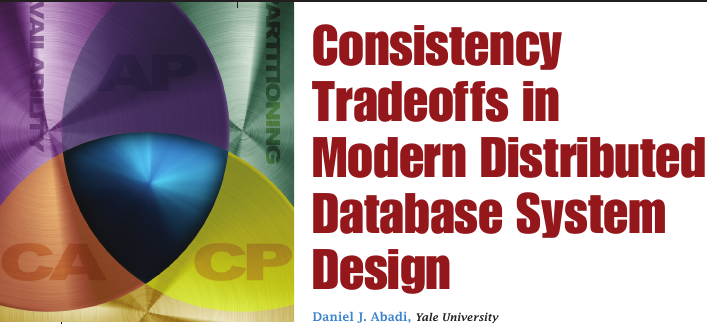
\includegraphics[scale = 0.25]{figs/pacelc-paper.png}};
  \node[above = of pacelc] (pacelc-fig) {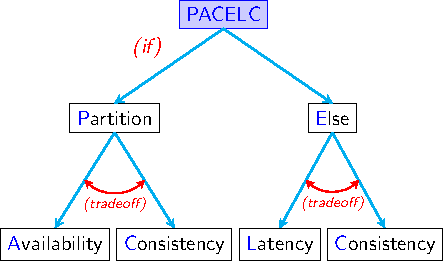
\includegraphics[scale = 0.80]{figs/pacelc-tradeoff-new.pdf}};
\end{tikzpicture}

%     \end{adjustbox}
%   \end{figure}
% \end{frame}
%%%%%%%%%%%%%%%
% \begin{frame}{数据一致性问题研究的历史阶段 (结论)}
%   \begin{columns}[T]
% 	\column{0.40\textwidth}
% 	  新平台, 新特点:
% 	  \vspace{0.30cm}
% 	  \begin{itemize}
% 		\item 更丰富的应用
% 		\item 更复杂的权衡
% 	  \end{itemize}
% 	\column{0.45\textwidth}
% 	\only<2->{更具\textcolor{brown}{``柔性''}的数据一致性理论:}
% 	  \vspace{0.30cm}
% 	  \begin{itemize}
% 		\item<3-> 多样化, 可调节
% 		\item<4-> 精细化, 可度量
% 	  \end{itemize}
%   \end{columns}
% \end{frame}

  % \uncover<1->{\textcolor{blue}{需要什么样的数据一致性理论?}}
  % \vspace{0.30cm}

  % \begin{columns}[t]
  %   \column{0.50\textwidth}
  %     \uncover<2->{
  %     (1) 
  %     } 
  %   \column{0.50\textwidth}
  %     \uncover<3->{
  %    (2) 体现更丰富的 tradeoffs
  %     \fignocaption{width = 0.60\textwidth}{figures/consistency-centric-tradeoff.pdf}
  %     }
  % \end{columns}
%%%%%%%%%%%%%%%
\begin{frame}{分布数据一致性问题研究理念 (I)}
  % \begin{center}
  %   \textcolor{red}{新平台, 新特点:} 更复杂的权衡、更丰富的应用
  % \end{center}
  \textcolor{red}{新平台, 新特点:} 

  \begin{itemize}
	\item<2-> 更复杂的权衡 $\Longrightarrow$ 正确性变得模糊 {\small (blurred)}
	\item<3-> 更丰富的应用 $\Longrightarrow$ 多样性变得重要
  \end{itemize}

  % \vspace{0.50cm}
  % \only<2>{
  % 棒球赛应用一致性需求~\citeinbeamer{Terry}{SOSP}{13}:
  % \begin{description}
  %   \item[记分员:] 采用 \textcolor{blue}{\texttt{\small read-my-writes consistency}} 更新比赛得分
  %   \item[电台记者:] 采用 \textcolor{blue}{\texttt{\small monotonic reads consistency}} 避免读到陈旧比分
  % \end{description}
  % }

  % \vspace{0.25cm}
  % \only<3>{
  % 出租车实时位置查询一致性需求:
  % \begin{description}
  %   \item[权衡:] 为了保证低延迟, 允许违反 \textcolor{blue}{\texttt{\small atomicity}}
  %   \item[有界:] 所有读请求都要满足 \textcolor{blue}{\texttt{\small 2-atomicity}}
  %   \item[量化需求:] 违反 \textcolor{blue}{\texttt{\small atomicity}} 的读请求低于$1\%$ 
  % \end{description}
  % }

  \vspace{1.00cm}
  \uncover<4->{
	\centerline{需要更具\textcolor{brown}{``柔性''}的分布数据一致性理论:}
  }
  \begin{description}
	\centering
	\item<5>[理念一:] 多样化, 可调节
	\item<5>[理念二:] 精细化, 可度量
  \end{description}
\end{frame}
%%%%%%%%%%%%%%%
\begin{frame}{数据一致性问题研究理念 (II)}
  \begin{description}
	\setlength{\itemsep}{10pt}
	\item[多样化:] 从单一到融合 (mono- vs. multi-) \citeinbeamer{Terry}{CACM}{13} 
	  \vspace{5pt}
	  \begin{itemize}
		\setlength{\itemsep}{5pt}
		\item 融合强弱一致性: 不同操作, 不同一致性需求 
		\item 融合一致与不一致: 容忍``有限度''的不一致
	  \end{itemize}
	  \begin{columns}
		\column{0.50\textwidth}
		  \fignocaption{width = 0.50\textwidth}{figures/tradeoff.jpg} 
		\column{0.50\textwidth}
		  \fignocaption{width = 0.35\textwidth}{figures/one-size-fit-all-text.jpg} 
	  \end{columns}
	\pause
	\item[可调节:] think \textcolor{red}{\it dynamically} \citeinbeamer{Terry}{SOSP}{13}
	  \vspace{10pt}
	  \begin{center}
	    依据应用需求/系统状态调节数据一致性
	  \end{center}
  \end{description}
\end{frame}
%%%%%%%%%%%%%%%
\begin{frame}{数据一致性问题研究理念 (III)}
  \begin{description}
	\setlength{\itemsep}{20pt}
	\item[精细化:] 从二元 {\small \;$\set{0,1}$} 到连续谱 {\small \;$(0,1)$}~\citeinbeamer{Yu}{TOCS}{02}
	  \begin{columns}
		\column{0.50\textwidth}
		  \fignocaption{scale = 0.15}{figures/black-or-white.jpg}
		\column{0.50\textwidth}
		  \fignocaption{scale = 0.05}{figures/prism-spectrum.jpg}
	  \end{columns}
	  \pause
	\item[可度量:] think \textcolor{red}{\it probabilistically} \citeinbeamer{Brewer}{PODC}{00}
	  \vspace{10pt}
	  \begin{center}
		度量系统满足一致性的程度
	  \end{center}
  \end{description}
\end{frame}
%%%%%%%%%%%%%%%
\begin{frame}{数据一致性问题研究理念 (IV)}
  \mdf{red}{red}{论文研究问题}{
	\begin{center}
	  如何面向大规模分布式系统研究\\能体现\idea{}\\理念的分布数据一致性技术?
	\end{center}
  }

  \pause

  \mdf{blue}{blue}{论文主要贡献}{
	\begin{description}
	  % \item<2->[理念:] 提出\idea{}的数据\\一致性问题研究理念
	  \item<2->[框架:] 提出包含``一个基础、三个维度''的技术框架 
	  \item<3->[VPC:] 验证 Pipelined-RAM Consistency \hfill \textcolor{brown}{\scriptsize [``精细化, 可度量'']}
	  \item<3->[PA2AM:]	量化 2-Atomicity 协议 \hfill \textcolor{brown}{\scriptsize [``精细化, 可度量'']} 
	  \item<3->[RVSI:] 可调节 Snapshot Isolation \hfill \textcolor{brown}{\scriptsize [``多样化, 可调节'']}
	\end{description}
  }
\end{frame}
%%%%%%%%%%%%%%%